\documentclass[11pt,a4paper,twoside]{report}
\usepackage{amsmath,titlesec}
\usepackage{paralist}
\usepackage[scaled]{beramono}
\usepackage{colortbl}
\definecolor{gray-5}{gray}{0.95}
\definecolor{gray-10}{gray}{0.9}
\definecolor{gray-20}{gray}{0.8}
\definecolor{gray-30}{gray}{0.7}
\definecolor{gray-40}{gray}{0.6}
\definecolor{fadered}{rgb}{0.988, 0.914, 0.310}
\usepackage{charter}
\usepackage{longtable}
\usepackage{multirow}
\usepackage{multicol}
\usepackage[pdftex]{graphicx}
\usepackage{caption}
\usepackage[top=1in, bottom=1in, left=1in, right=1in]{geometry}
\usepackage[charter]{mathdesign}
\usepackage[utf8]{inputenc}
% \usepackage[none]{hyphenat} 
\usepackage{natbib}
\usepackage{float}
\usepackage[final]{pdfpages}

\usepackage{sidecap}

\makeatletter
  \newenvironment{SCtopfig}{\SC@float[t]{figure}}{\endSC@float}
\makeatother

% \usepackage{setspace}
\usepackage[charter]{mathdesign}
% \usepackage[small]{caption}
% \usepackage{abstract}
% \usepackage{lineno}
\setlength{\headheight}{14pt}
\newcommand{\includepublication}[1]{\cleardoublepage\includepdf{#1}}
% \newcommand{\includepublication}[1]{}
\usepackage{nomencl}
\makenomenclature

\sloppy

\usepackage{listings} 
\lstset{numbers=left, numberstyle=\scriptsize\ttfamily, numbersep=10pt, captionpos=b} 
\lstset{backgroundcolor=\color{gray-5}}
\lstset{basicstyle=\small\ttfamily}
\lstset{framesep=4pt}
\lstset{language={}}
\newcommand{\inlineCode}{\lstinline[basicstyle=\normalsize\ttfamily]}
\newcommand{\first}[1]{{\vspace{1ex}}{\Large \textbf{#1}}{\vspace{1ex}}}
\newcommand{\second}[1]{{\vspace{1ex}}{\large \textbf{#1}}}
\newcommand{\tabspace}[0]{\vspace{2mm}}
\newcommand{\cvsubheader}[1]{\multicolumn{2}{@{}l}{\second{#1}} \\ \nopagebreak[4]}
\newcommand{\cvitem}[1]{\input{../../common/#1}}
\newcommand{\cvtitle}[2]{#1 & \textbf{#2} \\ \nopagebreak}
\renewcommand\bibname{References}

\usepackage[colorlinks=true,linkcolor=black,citecolor=black,urlcolor=black,filecolor=black,bookmarks=true]{hyperref}
\hypersetup{
pdfauthor = {Michael Specht},
pdftitle = {},
pdfsubject = {},
pdfkeywords = {},
pdfcreator = {LaTeX},
pdfproducer = {pdflatex}}

% 
    \makeatletter 
    \def\cleardoublepage{\clearpage\if@twoside \ifodd\c@page\else% 
    \hbox{}% 
    \thispagestyle{empty}
    \newpage% 
    \if@twocolumn\hbox{}\newpage\fi\fi\fi} 
    \makeatother

% Definition from latex.ltx modified
% \makeatletter
% \renewcommand*{\cleardoublepage}{%
%   \clearpage
%   \if@twoside
%     \ifodd\c@page
%       \hbox{}%
%       \newpage
%       \if@twocolumn
%         \hbox{}%
%         \newpage
%       \fi
%     \fi
%   \fi
% }
% \makeatother

\fboxsep0pt
\fboxrule0.05pt

\newcommand{\image}[5]{
  \begin{figure}[htbp]
    \centering
    \includegraphics[width=#3\textwidth]{#2}
    \caption[#5]{#4}
    \label{fig:#1}
  \end{figure}
}

\newcommand{\imageFrame}[5]{
  \begin{figure}[htbp]
    \centering
    \fbox{
      \includegraphics[width=#3\textwidth]{#2}
    }
    \caption[#5]{#4}
    \label{fig:#1}
  \end{figure}
}


\usepackage{setspace}
\usepackage{fancyhdr}
\usepackage{wrapfig}
% \renewcommand{\chaptermark}[1]{\markleft{#1}{}}
% \renewcommand{\sectionmark}[1]{\markright{#1}{}}
% \fancyhead[C]{\rightmark}
% \renewcommand{\headrulewidth}{0pt}
% \renewcommand{\footrulewidth}{0pt}
\def \cre{{\em C.~reinhardtii}}
\def \dmel{{\em D.~melanogaster}}
\def \chlre{{\em Chlamydomonas reinhardtii}}

\def \fmfour{FM4}
\def \augno{AUGUSTUS}
\def \augyes{AUGUSTUS/GPF}
\def \etal{{\em et al.}}
\def \denovo{{\em de novo}}
\def \insilico{{\em in silico}}
\def \mz{{\em m/z}}
\newcommand\caret{\mathbin{\char`\^}}

\hyphenation{AUGUSTUS}
\hyphenation{chro-ma-to-gra-phy}
\setlength{\parskip}{2mm}
\setlength{\parindent}{0mm}
\renewcommand{\baselinestretch}{1.4} 
\renewcommand{\arraystretch}{1.4} 

\renewcommand{\headrulewidth}{0.25pt}

% \pagestyle{fancy}

%\setlength{\marginparwidth}{1.5cm}
%\newcommand{\note}[1]{\marginpar{\color{gray-40}\footnotesize \flushleft #1}}
\newcommand{\note}[1]{}

\newcommand{\imageCourtesy}[2]{Image courtesy of #1 \cite{#2}.}

\lstnewenvironment{todo}{\lstset{numbers=none,frame=none,backgroundcolor=\color{fadered}}}{}
% \pagestyle{empty}

% Code for creating empty pages
% No headers on empty pages before new chapter
% \makeatletter
% \def\cleardoublepage{\clearpage\if@twoside \ifodd\c@page\else
%     \hbox{}
%     \thispagestyle{plain}
%     \newpage
%     \if@twocolumn\hbox{}\newpage\fi\fi\fi}
% \makeatother \clearpage{\pagestyle{plain}\cleardoublepage}


\renewcommand{\headrulewidth}{0.25pt}
\fancyhf{}
\fancyhead[EL,OR]{\thepage}
\renewcommand{\chaptermark}[1]{\markboth{#1}{}}
\renewcommand{\sectionmark}[1]{\markright{#1}}

\fancypagestyle{plain} {
    \renewcommand{\headrulewidth}{0.0pt}
    \fancyhf{}
    % \fancyhead[ER]{\leftmark}
    % \fancyhead[OL]{\rightmark}
}


% Code for creating empty pages
% No headers on empty pages before new chapter
\makeatletter
\def\cleardoublepage{\clearpage\if@twoside \ifodd\c@page\else
    \hbox{}
    \thispagestyle{plain}
    \newpage
    \if@twocolumn\hbox{}\newpage\fi\fi\fi}
\makeatother \clearpage{\pagestyle{plain}\cleardoublepage}

\begin{document}
\pagestyle{empty}
% \pagewiselinenumbers

\includepdfset{pages=-,noautoscale}

\begin{center}

\includegraphics[width=0.5\textwidth]{figures/wwu-logo-black.jpg}

{\Large Institut f\"ur Biologie und Biotechnologie der Pflanzen}

\vspace*{5cm}

% {\bf \Huge {\em Chlamydomonas reinhardtii} from the computational proteomics perspective}
{\bf \Huge Novel high-throughput data analysis strategies in computational proteomics and proteogenomics}

\vspace*{4cm}

{\Large Inaugural-Dissertation zur Erlangung des Doktorgrades der
Naturwissenschaften im Fachbereich Biologie der
Mathematisch-Naturwissenschaftlichen Fakult\"at der
\mbox{Westf\"alischen Wilhelms-Universit\"at M\"unster}}

\vspace*{2cm}

{\Large vorgelegt von}

{\LARGE \bf Michael Specht}

{\Large aus Magdeburg}

{\LARGE April 2011}

\end{center}

\cleardoublepage

\vspace*{550pt}

Dekan: Prof. Dr. Christian Kl\"ambt \newline
Erster Gutachter: Prof. Dr. Michael Hippler \newline
Zweite Gutachterin: Prof. Dr. Simone K\"onig \newline
Tag der m\"undlichen Pr\"ufung: \newline
Tag der Promotion: \newline

\cleardoublepage

\vspace*{200pt}
\begin{flushright}
{\Large\em
To my family, the great life amplifier: \\
Jule, Charlotte \& Leo
}
\end{flushright}

% \clearpage

% \begin{abstract}
% This is the abstract. Lots of hacking and MS here.
% \end{abstract}

% {\bf Abbreviations and acronyms used in the report:}
% 
% DSCAM -- down syndrome cell adhesion molecule, 
% FDR -- false discovery rate, 
% GPF -- Genomic Peptide Finder, 
% MS -- mass spectrometry,
% MS/MS -- tandem mass spectrometry,
% PSM -- peptide/spectral match

% \fancypagestyle{plain}{
% \fancyhf{}
% \renewcommand{\headrulewidth}{0.25pt}
% % \renewcommand{\footrulewidth}{0.5pt}
% \fancyfoot[EL,OR]{\thepage}
% \fancyhead[EL]{\leftmark}
% \fancyhead[OR]{\rightmark}
% }

\cleardoublepage
% \begin{multicols}{2}
\setlength{\nomlabelwidth}{0.15\hsize}
\printnomenclature
% \end{multicols}

\cleardoublepage

\setcounter{tocdepth}{1}
\setcounter{secnumdepth}{1}
\tableofcontents

\clearpage



\nomenclature{AMT}{accurate mass/time}
\nomenclature{CID}{collision-induced dissociation}
\nomenclature{CLI}{command-line interface}
\nomenclature{DIGE}{difference gel electrophoresis}
\nomenclature{DNA}{deoxyribonucleic acid}
\nomenclature{ESI}{electrospray ionization}
\nomenclature{EST}{expressed sequence tag}
\nomenclature{FDR}{false discovery rate}
\nomenclature{FT-ICR}{Fourier transform ion cyclotron resonance}
\nomenclature{GPF}{Genomic Peptide Finder}
\nomenclature{GUI}{graphical user interface}
\nomenclature{HPLC}{high performance liquid chromatography}
\nomenclature{ICAT}{isotope-coded affinity tag}
\nomenclature{iTRAQ}{isobaric tag for relative and absolute quantitation}
\nomenclature{LC}{liquid chromatography}
\nomenclature{MALDI}{matrix-assisted laser desorption/ionization}
\nomenclature{MS}{mass spectrometry}
\nomenclature{MS/MS}{tandem mass spectrometry}
\nomenclature{OMSSA}{Open mass spectrometry search algorithm}
\nomenclature{PSM}{peptide/spectral match}
\nomenclature{PTM}{post-translational modification}
\nomenclature{RNA}{ribonucleic acid}
\nomenclature{RPLC}{reverse phase liquid chromatography}
\nomenclature{SDS-PAGE}{sodium dodecyl sulfate polyacrylamide gel electrophoresis}
\nomenclature{TOF}{time of flight}

\clearpage

\pagestyle{fancy}
\renewcommand{\headrulewidth}{0.25pt}
\fancyhf{}
\fancyhead[EL,OR]{\thepage}
% \fancyhead[ER]{\leftmark}
% \fancyhead[OL]{\rightmark}
\renewcommand{\chaptermark}[1]{\markboth{#1}{}}
\renewcommand{\sectionmark}[1]{\markright{#1}}

\fancypagestyle{plain} {
    \renewcommand{\headrulewidth}{0.25pt}
    \fancyhf{}
    \fancyhead[EL,OR]{\thepage}
    % \fancyhead[ER]{\leftmark}
    % \fancyhead[OL]{\rightmark}
}

\cleardoublepage
% ==============================================================
\chapter{Introduction}
% ==============================================================

The availability of genome sequences is a key prerequisite for modern 
biological research.
After the discovery of the DNA double helix structure \citep{Watson1953},
genome sequencing techniques have been developed and refined over the decades
\citep{Gilbert1973, Sanger1975}, 
culminating in the publication of the full human genome sequence in 2001 
\citep{Venter2001}.
Aside from the ambiguities introduced by non-coding regions in the genome 
\citep{Gilbert1978} and alternative splicing of genes \citep{Black2003}, 
the genome provides, in theory, all necessary information about which proteins 
can potentially be expressed in a cell.
However, in order to study the dynamic nature of a cell or organism, as for 
example in response to changing environmental conditions, the static information
provided by the genome is not sufficient. 
The transcriptome provides information about gene expression at the RNA level. 
DNA microarray techniques can be employed to screen the regulation of many
genes in parallel on the transcript level \citep{Schena1995}.

Complementing transcriptomics, the field of proteomics deals with the total
set of proteins expressed in a cell, tissue, or organism, at a defined time
point and under certain conditions \citep{Yarmush2002, Yates2009}.
In contrast to transcriptomics, proteomics is situated at the stage of 
translation and protein synthesis, and therefore most accurately reflects the 
phenotype of a cell. 
Mass spectrometry provides an excellent means for proteome analysis
\citep{Aebersold2003}, with speed, accuracy, and sensivity rapidly increasing
within the past two decades.
The major goals of mass spectrometry-based proteomics are protein 
identification and quantitation.
However, since most proteins are too heavy to be measured directly, the
analysis is usually performed on the peptide level, with proteins being digested
prior to the measurement using proteolytic enzymes such as Trypsin, Lys-C, or 
Pepsin. 
The inherent ambiguity introduced by protein isoforms or alternative splicing
poses an additional challenge when peptide identifications are shifted to
the protein level.
In addition to the raw amino acid sequence encoded by a gene, post-translational
modifications play an important role in defining the actual function of a
protein.
Post-translational modifications may modify a protein by adding an enzyme or by
chemically modifying certain residues.
Furthermore, structural adjustments such as the formation of disulfide 
bonds between Cysteine residues may be required for the protein to become 
functional.
Employing mass spectrometry, it is possible not only to identify peptides and
proteins, but also to study their various modifications.
Another application of mass spectrometry-based analysis is the localization of
proteins to certain compartments of a cell, for example by semi-quantitative
analysis.

Although modern mass spectrometers are very sensitive, a couple of sample 
preparation steps must be carried out in order to achieve comprehensive 
proteome coverage. 
An example of a mass spectrometry-based proteomics workflow for peptide 
and protein identification is depicted in Fig.~\ref{fig:proteomics-overview}.

\begin{figure}
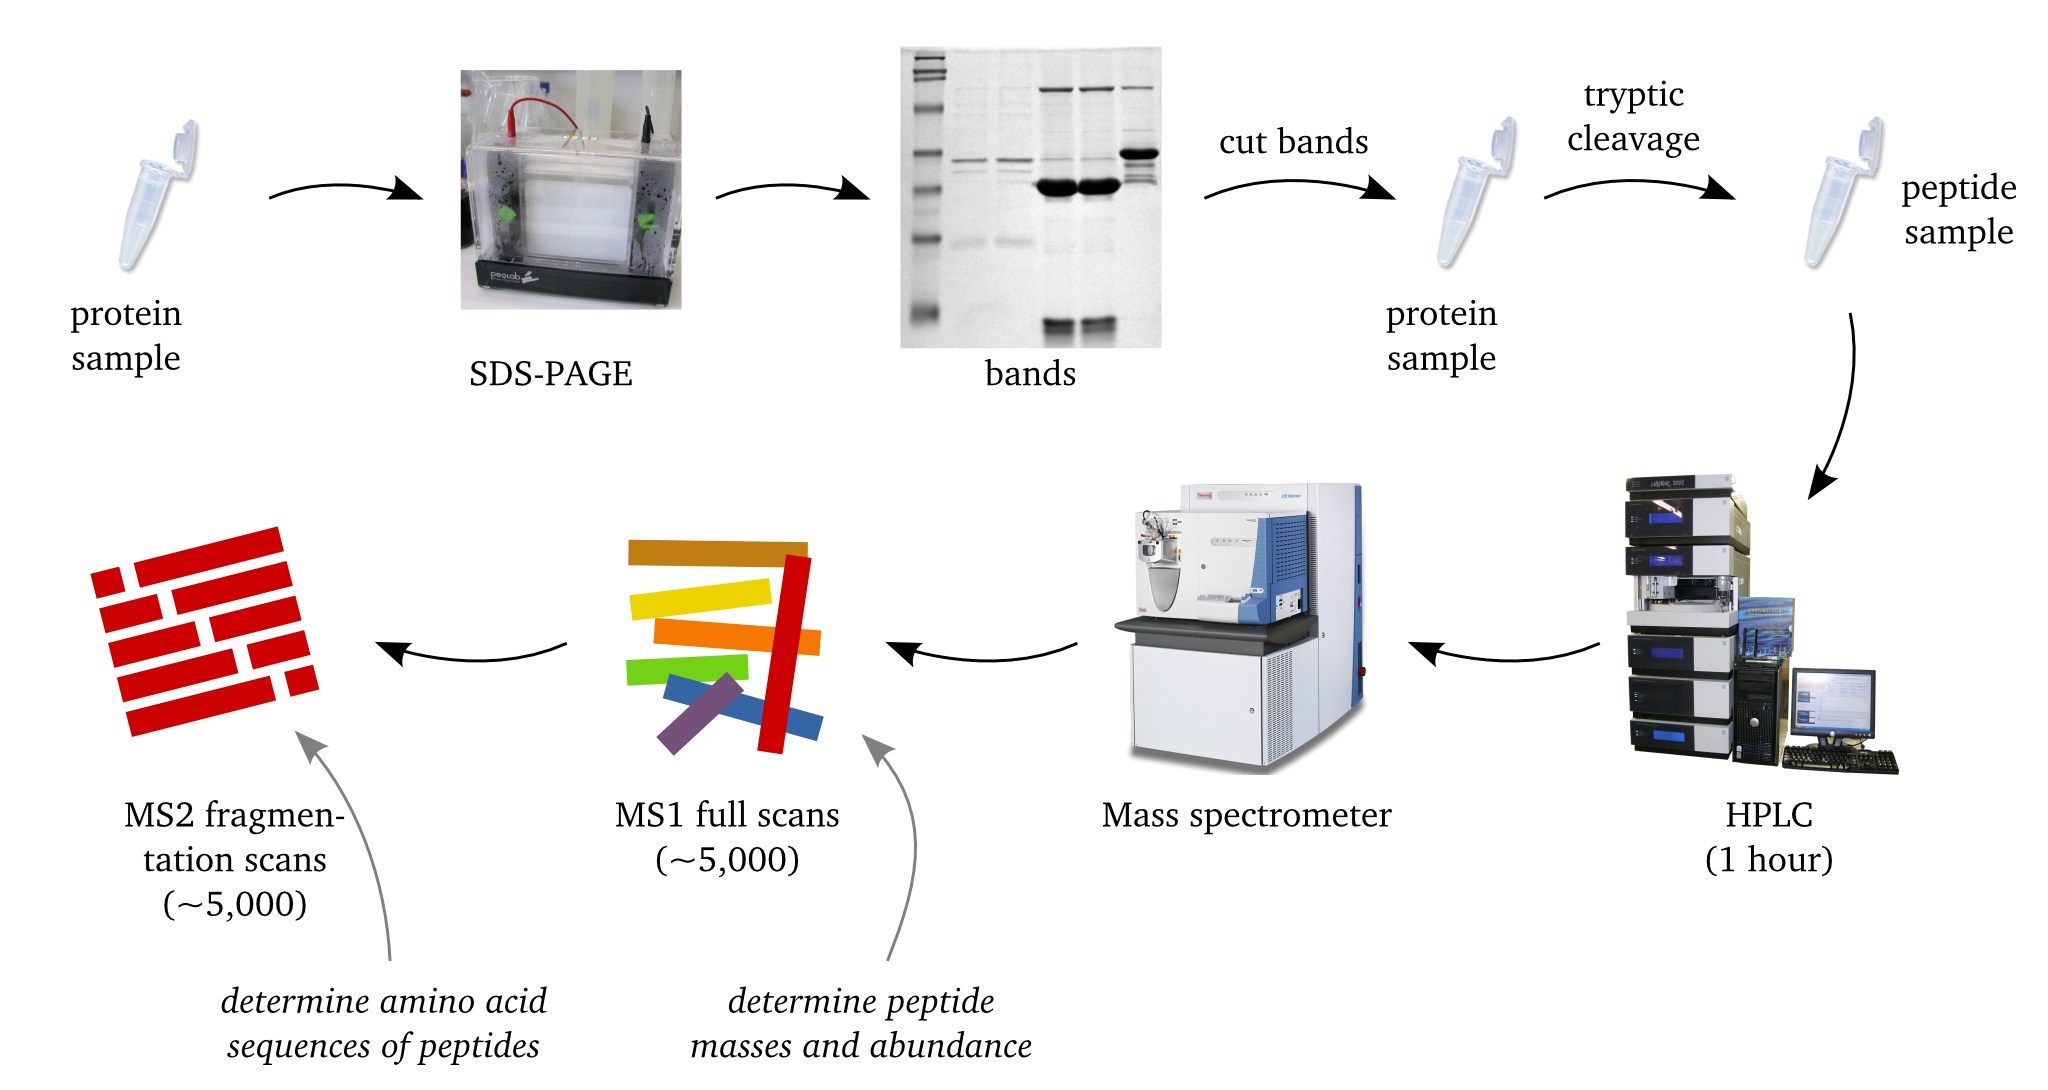
\includegraphics[width=\textwidth]{figures/Proteomics.jpg}
\caption{
{\bf Example of a mass spectrometry-based proteomics experiment workflow.} 
Protein samples are fractionated via SDS-PAGE and resulting bands are excised and
digested proteolytically. In order to further separate the complex mixture, 
the resulting peptides are loaded onto a HPLC column and subsequently eluted 
and injected into the mass spectrometer. Full scans and fragmentation scans
are recorded as peptide elution is in progress for a pre-defined amount of time.
}
\label{fig:proteomics-overview}
\end{figure}

% --------------------------------------------------------------
\section{Acquisition of mass spectrometric data}
% --------------------------------------------------------------

In the following, the steps involved in the acquisition of mass spectrometric
data are described.

\subsection{Preprocessing of biological samples}

Although mass spectrometric analysis of intact proteins has been successfully
reported \citep{Lee2002, Taylor2003}, such an approach is not feasible in 
general because the high mass of proteins cannot be accounted for with most
types of mass spectrometers.
In addition, low abundant proteins may be missed in complex samples due to
the fact that there are many more highly abundant proteins present.
To overcome these obstacles, a couple of sample preprocessing steps are usually
undertaken, with possible variations depending on the experimental context.

\subsubsection{Gel electrophoresis}

Due to the high dynamic range of protein expression levels, complex protein 
mixtures tend to produce less comprehensive results because low abundant 
proteins are `shadowed' by highly abundant proteins. 
Gel electrophoresis may be used as a first sample separation step in which
proteins are ordered by size, resulting in a number of fractions which can
be analyzed individually.
For SDS-PAGE, a sodium dodecyl sulfate polyacrylamide gel is prepared and
proteins are loaded into wells in the gel.
An electric field is applied to the gel, thus inducing an electromotive force 
on the proteins which move through the gel at a speed which depends on their
size and charge.
However, SDS leads to denaturation of proteins and results in an overall
negative charge for all proteins. 
Thus, the migration speed of the proteins is only dependent on their size. 
Individual spots of equally-sized proteins may be visualized using Coomassie 
dye and subsequently excised.

In order to achieve even higher sample separation, two-dimensional gel 
electrophoresis may be used \citep{Klose1975, O'Farrell1975}.
Here, proteins are additionally separated by a second physicochemical property
such as their isoelectric point.
As in the SDS-PAGE approach, resulting spots may be excised and subjected 
to mass spectrometric analysis.

\subsubsection{Proteolysis}

In order to break proteins up into small, mass spectrometry-compatible peptides, 
proteolytic enzymes are used.
Among the various choices of possible enzymes, Trypsin has become very popular
because it results in short peptides with a basic residue at the C-terminus
\citep{Olsen2004}.
Trypsin cleaves specifically at the C-terminal side of Lysine and Arginine 
residues, given that no Proline residue is located at the other side of the 
cleavage site.
Alternative enzymes such as Asp-N and Glu-C are sometimes used to generate
complementing peptides which overlap with the tryptic peptides in order to 
increase sequence coverage of peptide identifications \citep{Steen2004}.
Although Trypsin, Asp-N and Glu-C are very sequence-specific, the possibility 
of missed cleavage sites must be taken into account during data analysis.

\subsubsection{Liquid chromatography}

In addition to fractionation via SDS-PAGE, liquid chromatography (LC) provides 
a second dimension of separation, usually at the peptide level.
For the experiments covered in this thesis, a reverse phase liquid 
chromatography (RPLC) system has been employed.
In this setup, peptide elute according to their hydrophobicity.

\subsection{Ionization of molecules}

\begin{todo}
ESI, MALDI
\end{todo}

\subsection{Mass analysis and ion detection}

\begin{todo}
separation of ions by electromagnetic fields
TOF, Quadrupole, Ion traps (3D Quadrupole, Linear Quadrupole, Orbitrap), FT-ICR
\end{todo}

\begin{todo}
measure abundance of ions
\end{todo}

\subsection{Mass spectra}

Recorded mass spectra are stored as vendor-specific files which contain meta 
information which describes the acquired data as well as the raw peak data.
In order to unify the exchange of mass spectrometers raw data, the mzML file 
format has been devised by the HUPO Proteomics Standards Initiative
\citep{Deutsch2008}.
Apart from the file format details, several different scan types can be
acquired, each of which contains different information.

\subsubsection{Full scans (MS)}

Full scans provide an overview over the peptides which are present in the
mass spectrometer at a given time (see Fig.~\ref{fig:full-scan}).
The \mz~values of all intact peptides are reported.
However, the absence of a precursor peak does not necessarily indicate the
absence of the corresponding peptide in the sample, because detection of
an ion may fail for various reasons.
Following a full scan, one or more highly abundant precursors are usually
selected for further analysis.

\begin{figure}[h]
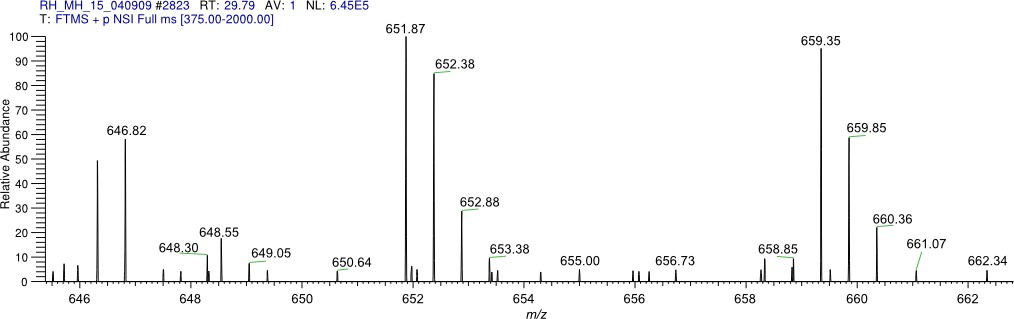
\includegraphics[width=\textwidth]{figures/ms1-scan.jpg}
\caption{
{\bf Zoomed view of a full scan.}
Isotope envelopes of doubly charged peptides, consisting of precursor
peaks with a \mz~difference of $\sim0.5$ are visible,
}
\label{fig:full-scan}
\end{figure}

\subsubsection{Fragmentation scans (MS/MS)}

Each of the selected ions gets fragmented in a process called
{\em collision induced dissociation} (CID), in which peptides collide with an
inert gas and subsequently break apart into N- and C-terminal fragments,
thereby producing {\em b} ions and {\em y} ions, respectively. 
Depending on the actual fragmentation site within the peptide bond,
alternative fragment ions may result: {\em a} and {\em c} ions for N-terminal
fragments, {\em x} and {\em z} ions for C-terminal fragments.
The resulting scan is called a fragmentation scan, or tandem MS (MS/MS) scan.

\begin{figure}[h]
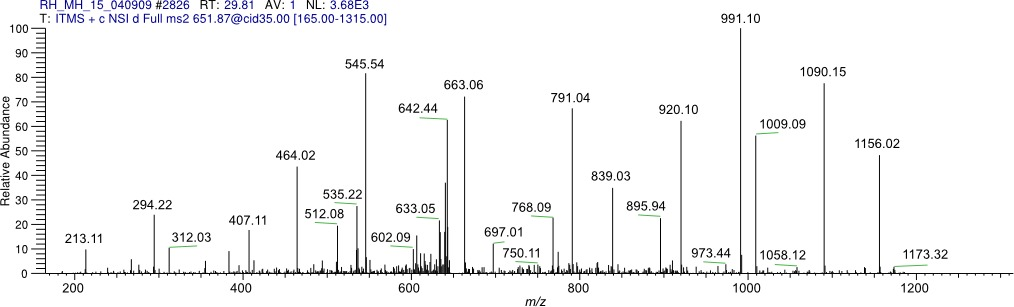
\includegraphics[width=\textwidth]{figures/ms2-scan.jpg}
\caption{
{\bf Example of a fragmentation scan.} 
The 651.87 \mz~precursor peak shown in Fig.~\ref{fig:full-scan} has been
subjected to collision-induced dissociation.
Resulting fragment ions are recorded in the fragmentation scan.
}
\label{fig:fragmentation-scan}
\end{figure}

From the observed fragment ions, {\em mass ladders} can be constructed which
represent the amino acid sequence of the selected peptide (see Fig~\ref{fig:fragmentation-scan-b-y}). 
When fragmentation peaks are missing, the exact sequence of the peptide may not
become clear from a single mass ladder.
However, a combination of multiple mass ladders can resolve such ambiguities.

\begin{figure}[h]
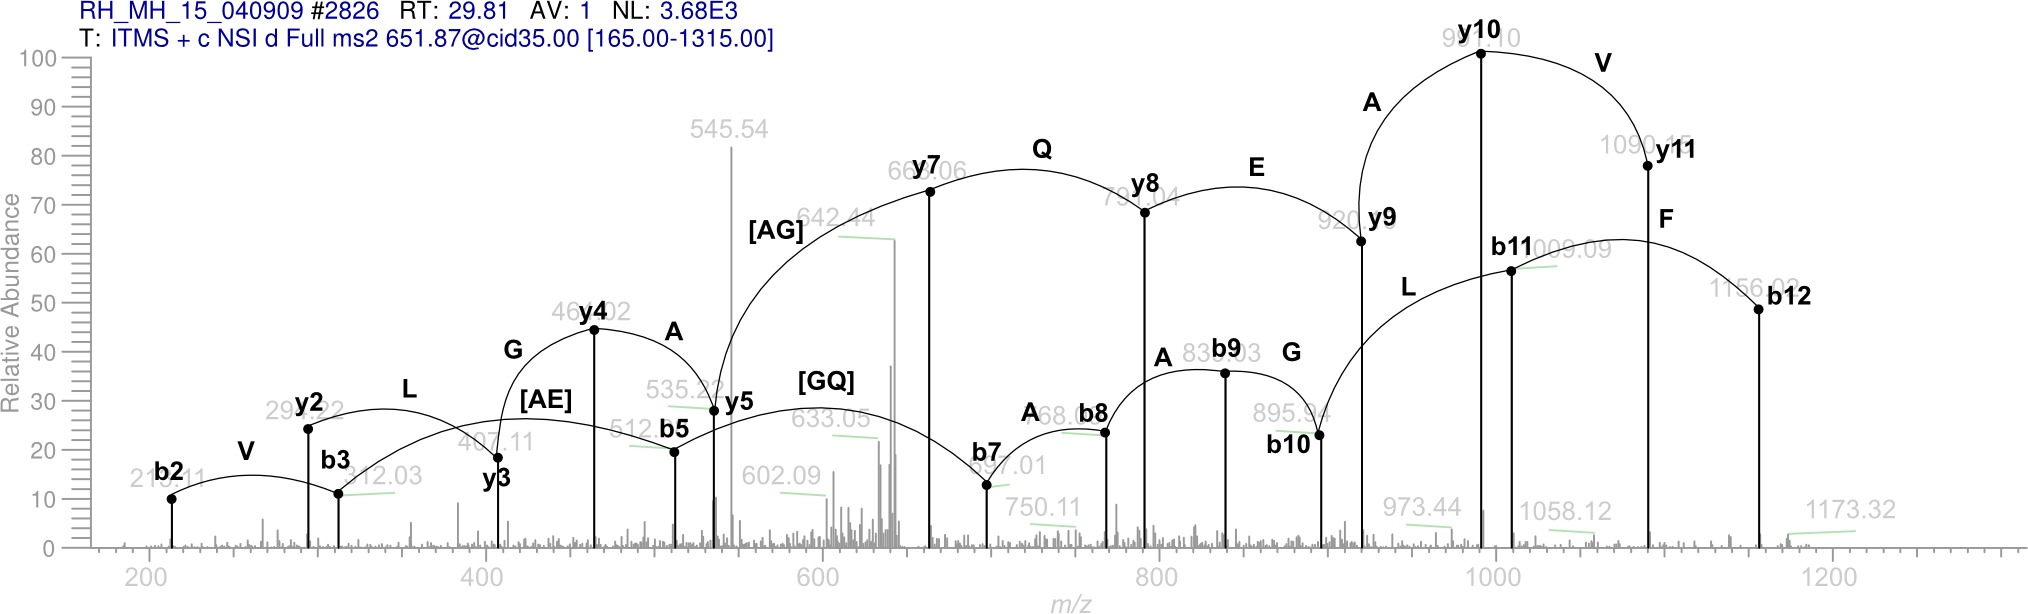
\includegraphics[width=\textwidth]{figures/ms2-scan-b-y-1.jpg}
\caption{
{\bf The MS/MS scan depicted in Fig.~\ref{fig:fragmentation-scan} with {\em b} and 
{\em y} ion series mass ladders superimposed.} 
The \mz~differences of fragmentation peaks reflect the masses of individual amino
acids or short amino acid oligomers.
}
\label{fig:fragmentation-scan-b-y}
\end{figure}


% --------------------------------------------------------------
\section{Data evaluation}
% --------------------------------------------------------------

Evaluation of the acquired mass spectrometric data is a process with a multitude
of possible options.
Usually, the decisions made during sample preparation and data acquisition are
reflected in the data analysis: If proteins were separated via SDS-PAGE, the
resulting order of proteins via their mass can be used to verify or falsify 
identifications.
Likewise, if liquid chromatography is employed, the retention time at which
peptides have been identified can be used for plausibility checks.

\subsection{Sequence databases}

Sequence databases, including genome and protein sequences, play an important
role in MS/MS data evaluation because they greatly confine the search space
for peptide identification from MS/MS spectra.
However, care must be taken if these databases are not comprehensive, because
the search space defined by incomplete sequence databases might be too small
to provide for proper identification.

\subsubsection{Genome annotation}

Genome sequence databases are a prerequisite for the prediction of protein 
databases, and full genome sequences for more than 180 species are available
\citep{Yates2009}.
The annotation of genomic sequences remains a challenge, especially in
eukaryotic genomes, where protein coding sequences are interrupted by
introns.
% EST support
Various strategies have been proposed to identify protein coding genes in
genomic sequences using expressed sequence tags (EST) libraries, 
including the UCSC KG II \citep{Karolchik2003}, ENSEMBL \citep{Hubbard2005} 
and NCBI Gnomon annotation pipelines \citep{Maglott2005}.
In this method, genes are identified by mapping known cDNA tags to the
genomic DNA sequence.
Consequently, high cDNA coverage is required to achieve comprehensive
genome annotation and therefore, low expressed transcripts pose a challenge.
% comparative
When cDNA information is unavailable, information from closely related
species can also be used for genome annotation.
Several software tools which implement this approach are available,
including TWINSCAN \citep{Korf2001}, SGP 2 \citep{Parra2003}, and 
SLAM \citep{Cawley2003}.

As an alternative to cDNA and conservation supported genome annotation,
{\em ab initio} genome annotation can be used for species for which no
or only little cDNA evidence is available and no closely related annotated
species exists.
In this approach, statistical calculations are performed on the genomic
DNA sequence, assessing various properties such as codon usage and splice 
site consensus sequences.
This approach allows for the initial annotation of novel genomic DNA 
sequences.
Programs using this approach include GENESCAN \citep{Burge1997}, 
GENEID \citep{Parra2000}, and AUGUSTUS \citep{Stanke2004, Stanke2006}.
In addition, the initial unbiased {\em ab initio} genome annotation can be 
supplemented with extrinsic information as it becomes available 
\citep{Stanke2008}.

\subsubsection{Proteogenomics}

\begin{todo}
genome annotation/gene model prediction, AUGUSTUS, external hints, 
EGASP, exon splice graph, GPF
\end{todo}

\subsection{Identification}

\subsubsection{Peptide mass fingerprinting}

\begin{todo}
sets of proteotypic precursor masses
\end{todo}

\subsubsection{Database search}

\begin{todo}
in silico digestion and matching via cross correlation or OMSSA-type & whatnot
\end{todo}

\subsubsection{De novo sequencing}

\begin{todo}
unbiased sequences, quite ambiguous, GPF by Jens Allmer
\end{todo}

\subsection{Quantitation}

\subsubsection{Chemical labeling}
 
\begin{todo}
ICAT, iTRAQ
\end{todo}

\subsubsection{Metabolic labeling}

\begin{todo}
SILAC, 15N
\end{todo}

\subsubsection{Label-free quantitation}

\begin{todo}
across several runs
\end{todo}

% --------------------------------------------------------------
\section{Chlamydomonas reinhardtii}
% --------------------------------------------------------------

\begin{todo}
soil or freshwater green alga, unicellular, hetertroph / photoautotrop, sexual & asexual
\end{todo}

\subsection{Anaerobic metabolism}

\begin{todo}
hydrogen production
\end{todo}

% --------------------------------------------------------------
\section{Thalassiosira oceanica}
% --------------------------------------------------------------

\begin{todo}
deep water diatom
\end{todo}

\subsection{Iron deficiency}

\begin{todo}
hydrogen production
\end{todo}


% \cleardoublepage
\cleardoublepage
% ==============================================================
\chapter{Specific aims}
% ==============================================================

The vast amounts of data acquired in large-scale mass spectrometric experiments
require software systems which are powerful enough to perform data evaluation
in a way which is fast enough and does not represent a potential bottleneck in 
the experimental data evaluation workflow.
Therefore, the available systems which provide mass-spectrometric data 
evaluation platforms to researchers require further improvement.
Most importantly, a decentralized setup which supports all common types of 
operating systems can be expected to allow for increased and data processing 
throughput at minimal cost because commodity hardware can be employed.
Furthermore, the utilization of the various software tools needs to be further 
facilitated.
The described platform should be able to provide all necessary tools for
the evaluation of MS/MS data, including protein identification and quantitation.
The design of the system should be flexible and general enough to also
allow the incorporation of tools which are outside the scope of mass 
spectrometry, such as genomics or structural bioinformatics.

With such a decentralized MS/MS data evaluation system available, the
characterization of the chloroplast proteome in \cre~will be performed using
semi-quantitative analysis.
Furthermore, an analysis of the anaerobic response of the chloroplast proteome
will be carried out, employing SILAC as a labeling strategy.
In order to carry out these analyses, specialized software for the 
high-throughput analysis of SILAC samples is required which is presented 
in this thesis.

The existing implementation of the Genomic Peptide Finder needs to
be improved in terms of search speed and sensitivity.
Another issue to be resolved is the statistical validation of GPF peptide 
assignments to MS/MS spectra.
Finally, the question arises whether peptides identified via {\em de novo} 
prediction and subsequent matching to the genome via the Genomic Peptide Finder 
can be used to establish a high-throughput proteogenomic genome annotation 
of \cre.
% It will be shown in this thesis that GPF-supported proteogenomic annotation 
% using high-throughput mass spectrometric data is feasible.


% \cleardoublepage
\cleardoublepage
% ==============================================================
\chapter{Publications}
% ==============================================================

The following publications are presented in this thesis:

\begin{enumerate}
\item 
{\bf Proteomics to go: Proteomatic enables the user-friendly creation of versatile MS/MS data evaluation workflows.}

Michael Specht, Sebastian Kuhlgert, Christian Fufezan and Michael Hippler

Bioinformatics (2011) 27 (8): 1183-1184; doi: \href{http://dx.doi.org/10.1093/bioinformatics/btr081}{10.1093/bioinformatics/btr081}.

\item
{\bf Characterizing the anaerobic response of Chlamydomonas reinhardtii by quantitative proteomics.}

Mia Terashima, Michael Specht, Bianca Naumann-Busch and Michael Hippler

Mol Cell Proteomics, 9(7), 2010: 1514-32; doi: \href{http://dx.doi.org/10.1074/mcp.M900421-MCP200}{10.1074/mcp.M900421-MCP200}.

\item
{\bf The chloroplast proteome: A survey from the {\em Chlamydomonas reinhardtii} perspective with a focus on distinctive features.}

Mia Terashima, Michael Specht and Michael Hippler

Current Genetics (2011), in press.

\item
{\bf Concerted action of the new Genomic Peptide Finder and AUGUSTUS allows for automated proteogenomic annotation of the {\em Chlamydomonas reinhardtii} genome.}

Michael Specht, Mario Stanke, Mia Terashima, Bianca Naumann-Busch, Ingrid Janßen, Ricarda H\"ohner, Erik F.~Y.~Hom, Chun Liang and Michael Hippler

Proteomics (2011), in press; doi: \href{http://dx.doi.org/10.1002/pmic.201000621}{10.1002/pmic.201000621}.

% \item
% {\bf T. oceanica paper with Markus Lommer}
% 
\item
{\bf p3d -- Python module for structural bioinformatics}

Christian Fufezan and Michael Specht

BMC Bioinformatics (2009) 10:258; doi: \href{http://dx.doi.org/10.1186/1471-2105-10-258}{10.1186/1471-2105-10-258}.

\end{enumerate}

% --------------------------------------------------------------
\cleardoublepage
\section{Proteomics to go: Proteomatic enables the user-friendly creation of versatile MS/MS data evaluation workflows}
% \markboth{Proteomics to go: Proteomatic enables the user-friendly creation of versatile MS/MS data evaluation workflows}{Proteomics to go: Proteomatic enables the user-friendly creation of versatile MS/MS data evaluation workflows}
% \addcontentsline{toc}{section}{Proteomics to go: Proteomatic enables the user-friendly creation of versatile MS/MS data evaluation workflows}

Michael Specht, Sebastian Kuhlgert, Christian Fufezan and Michael Hippler

Bioinformatics (2011) 27 (8): 1183-1184; doi: \href{http://dx.doi.org/10.1093/bioinformatics/btr081}{10.1093/bioinformatics/btr081}.

\subsection*{Contributions}

\begin{itemize}
\item design and implementation of the software system (Proteomatic)
\item manuscript writing
\item figure creation
\end{itemize}

% \cleardoublepage
\includepublication{publications/proteomatic-2011.pdf}

% --------------------------------------------------------------
\cleardoublepage
\section{Characterizing the anaerobic response of {\em Chlamydomonas reinhardtii} by quantitative proteomics}
% \markboth{Characterizing the anaerobic response of {\em Chlamydomonas reinhardtii} by quantitative proteomics}{Characterizing the anaerobic response of {\em Chlamydomonas reinhardtii} by quantitative proteomics}
% \addcontentsline{toc}{section}{Characterizing the anaerobic response of {\em Chlamydomonas reinhardtii} by quantitative proteomics}
% --------------------------------------------------------------

Mia Terashima, Michael Specht, Bianca Naumann-Busch and Michael Hippler

Mol Cell Proteomics, 9(7), 2010: 1514-32; doi: \href{http://dx.doi.org/10.1074/mcp.M900421-MCP200}{10.1074/mcp.M900421-MCP200}.

\subsection*{Contributions}

\begin{itemize}
\item design and implementation of the quantitation software (qTrace)
\item data evaluation
\item manuscript writing
\item figure creation
\end{itemize}

% \cleardoublepage
\includepublication{publications/terashima-2010.pdf}

% --------------------------------------------------------------
\cleardoublepage
\section{The chloroplast proteome: A survey from the {\em Chlamydomonas reinhardtii} perspective with a focus on distinctive features}
% \markboth{The chloroplast proteome: A concise survey form the {\em Chlamydomonas reinhardtii} perspective}{The chloroplast proteome: A concise survey form the {\em Chlamydomonas reinhardtii} perspective}
% \addcontentsline{toc}{section}{The chloroplast proteome: A concise survey form the {\em Chlamydomonas reinhardtii} perspective}
% --------------------------------------------------------------

Mia Terashima, Michael Specht and Michael Hippler

Current Genetics (2011), in press.

\subsection*{Contributions}

\begin{itemize}
\item data evaluation (BLAST analysis)
\item manuscript writing
\item figure creation
\end{itemize}

% \cleardoublepage
\includepublication{publications/terashima-2011-ms.pdf}

% --------------------------------------------------------------
\cleardoublepage
\section{Concerted action of the new Genomic Peptide Finder and AUGUSTUS allows for automated proteogenomic annotation of the {\em Chlamydomonas reinhardtii} genome}
% \markboth{Concerted action of the new Genomic Peptide Finder and AUGUSTUS allows for automated proteogenomic annotation of the {\em Chlamydomonas reinhardtii} genome}{Concerted action of the new Genomic Peptide Finder and AUGUSTUS allows for automated proteogenomic annotation of the {\em Chlamydomonas reinhardtii} genome}
% \addcontentsline{toc}{section}{Concerted action of the new Genomic Peptide Finder and AUGUSTUS allows for automated proteogenomic annotation of the {\em Chlamydomonas reinhardtii} genome}
% --------------------------------------------------------------

Michael Specht, Mario Stanke, Mia Terashima, Bianca Naumann-Busch, Ingrid Janßen, Ricarda H\"ohner, Erik F.~Y.~Hom, Chun Liang and Michael Hippler

Proteomics (2011), in press; doi: \href{http://dx.doi.org/10.1002/pmic.201000621}{10.1002/pmic.201000621}.

\label{paper:gpf}

\subsection*{Contributions}

\begin{itemize}
\item re-design and re-implementation of the software (GPF)
\item data evaluation
\item manuscript writing
\item figure creation
\end{itemize}

\cleardoublepage
\includepublication{publications/gpf-2011.pdf}

% % --------------------------------------------------------------
% \cleardoublepage
% \section{T.~oceanica paper with Markus Lommer}
% % \markboth{T.~oceanica paper with Markus Lommer}{T.~oceanica paper with Markus Lommer}
% % \addcontentsline{toc}{section}{T.~oceanica paper with Markus Lommer}
% % --------------------------------------------------------------
% 
% \subsection*{Contributions}
% 
% \begin{itemize}
% \item what was it, then?
% \end{itemize}
% 
% % \includepublication{publications/lommer-2011.pdf}

% --------------------------------------------------------------
\cleardoublepage
\section{p3d -- Python module for structural bioinformatics}
% \markboth{p3d -- Python module for structural bioinformatics}{p3d -- Python module for structural bioinformatics}
% \addcontentsline{toc}{section}{p3d -- Python module for structural bioinformatics}
% --------------------------------------------------------------

Christian Fufezan and Michael Specht

BMC Bioinformatics (2009) 10:258; doi: \href{http://dx.doi.org/10.1186/1471-2105-10-258}{10.1186/1471-2105-10-258}.

\subsection*{Contributions}

\begin{itemize}
\item implementation of the query parser module
\item speed optimization of spatial queries
\end{itemize}

% \cleardoublepage
\includepublication{publications/fufezan-2009.pdf}


% \cleardoublepage
% ==============================================================
\chapter{Discussion and outlook}
% ==============================================================

\section{Decentralized MS/MS data evaluation infrastructure}

\subsection{High-throughput data processing}

\subsection{Rapid deployment of novel functionality}

\section{Automated quantitation of metabolically labeled samples}

One of the studies presented in this thesis provides a comprehensive list of 
experimentally deduced chloroplast proteins for \cre~for the first time.
In addition, the anaerobic response of the chloroplast proteome of the green 
alga is characterized. 
Among other results, the induction of hydrogenase, a protein involved in 
hydrogen production, is confirmed \citep{Terashima2010}.

\section{Advancement of the Genomic Peptide Finder }

In 2007, GPF was redesigned and implemented from scratch in the scope of this
thesis to add a variety of features \citep{Specht2011_GPF}:

\begin{itemize}
\item intron splits may occur within a single coding nucleotide triplet
\item splice donor/acceptor site consensus sequences may be specified to
reduce the number of spurious spliced peptide alignments
\item increased search speed by employing an indexing strategy while locating
the occurences of sequence tags in the genomic DNA sequence
\end{itemize}

In addition, a method for the automated validation of GPF candidate peptides,
employing standard database search programs such as OMSSA was established.
This allows for statistically robust identification of GPF-deduced peptides
alongside gene model peptides.
Furthermore, an annotation pipeline was established in which resulting GPF
peptides are passed to AUGUSTUS, which performs an {\em ab initio} gene 
model prediction supplemented by various extrinsic hint sources including
GPF peptides.
It is therefore a major contribution of this thesis that an automated
proteogenomic annotation of the \cre~genome in which MS/MS data generated
for various unrelated purposes can be re-used for the generation of
extrinsic AUGUSTUS hints has become possible.

\paragraph{GPF-supported proteogenomic genome annotation.}

\begin{SCtopfig}
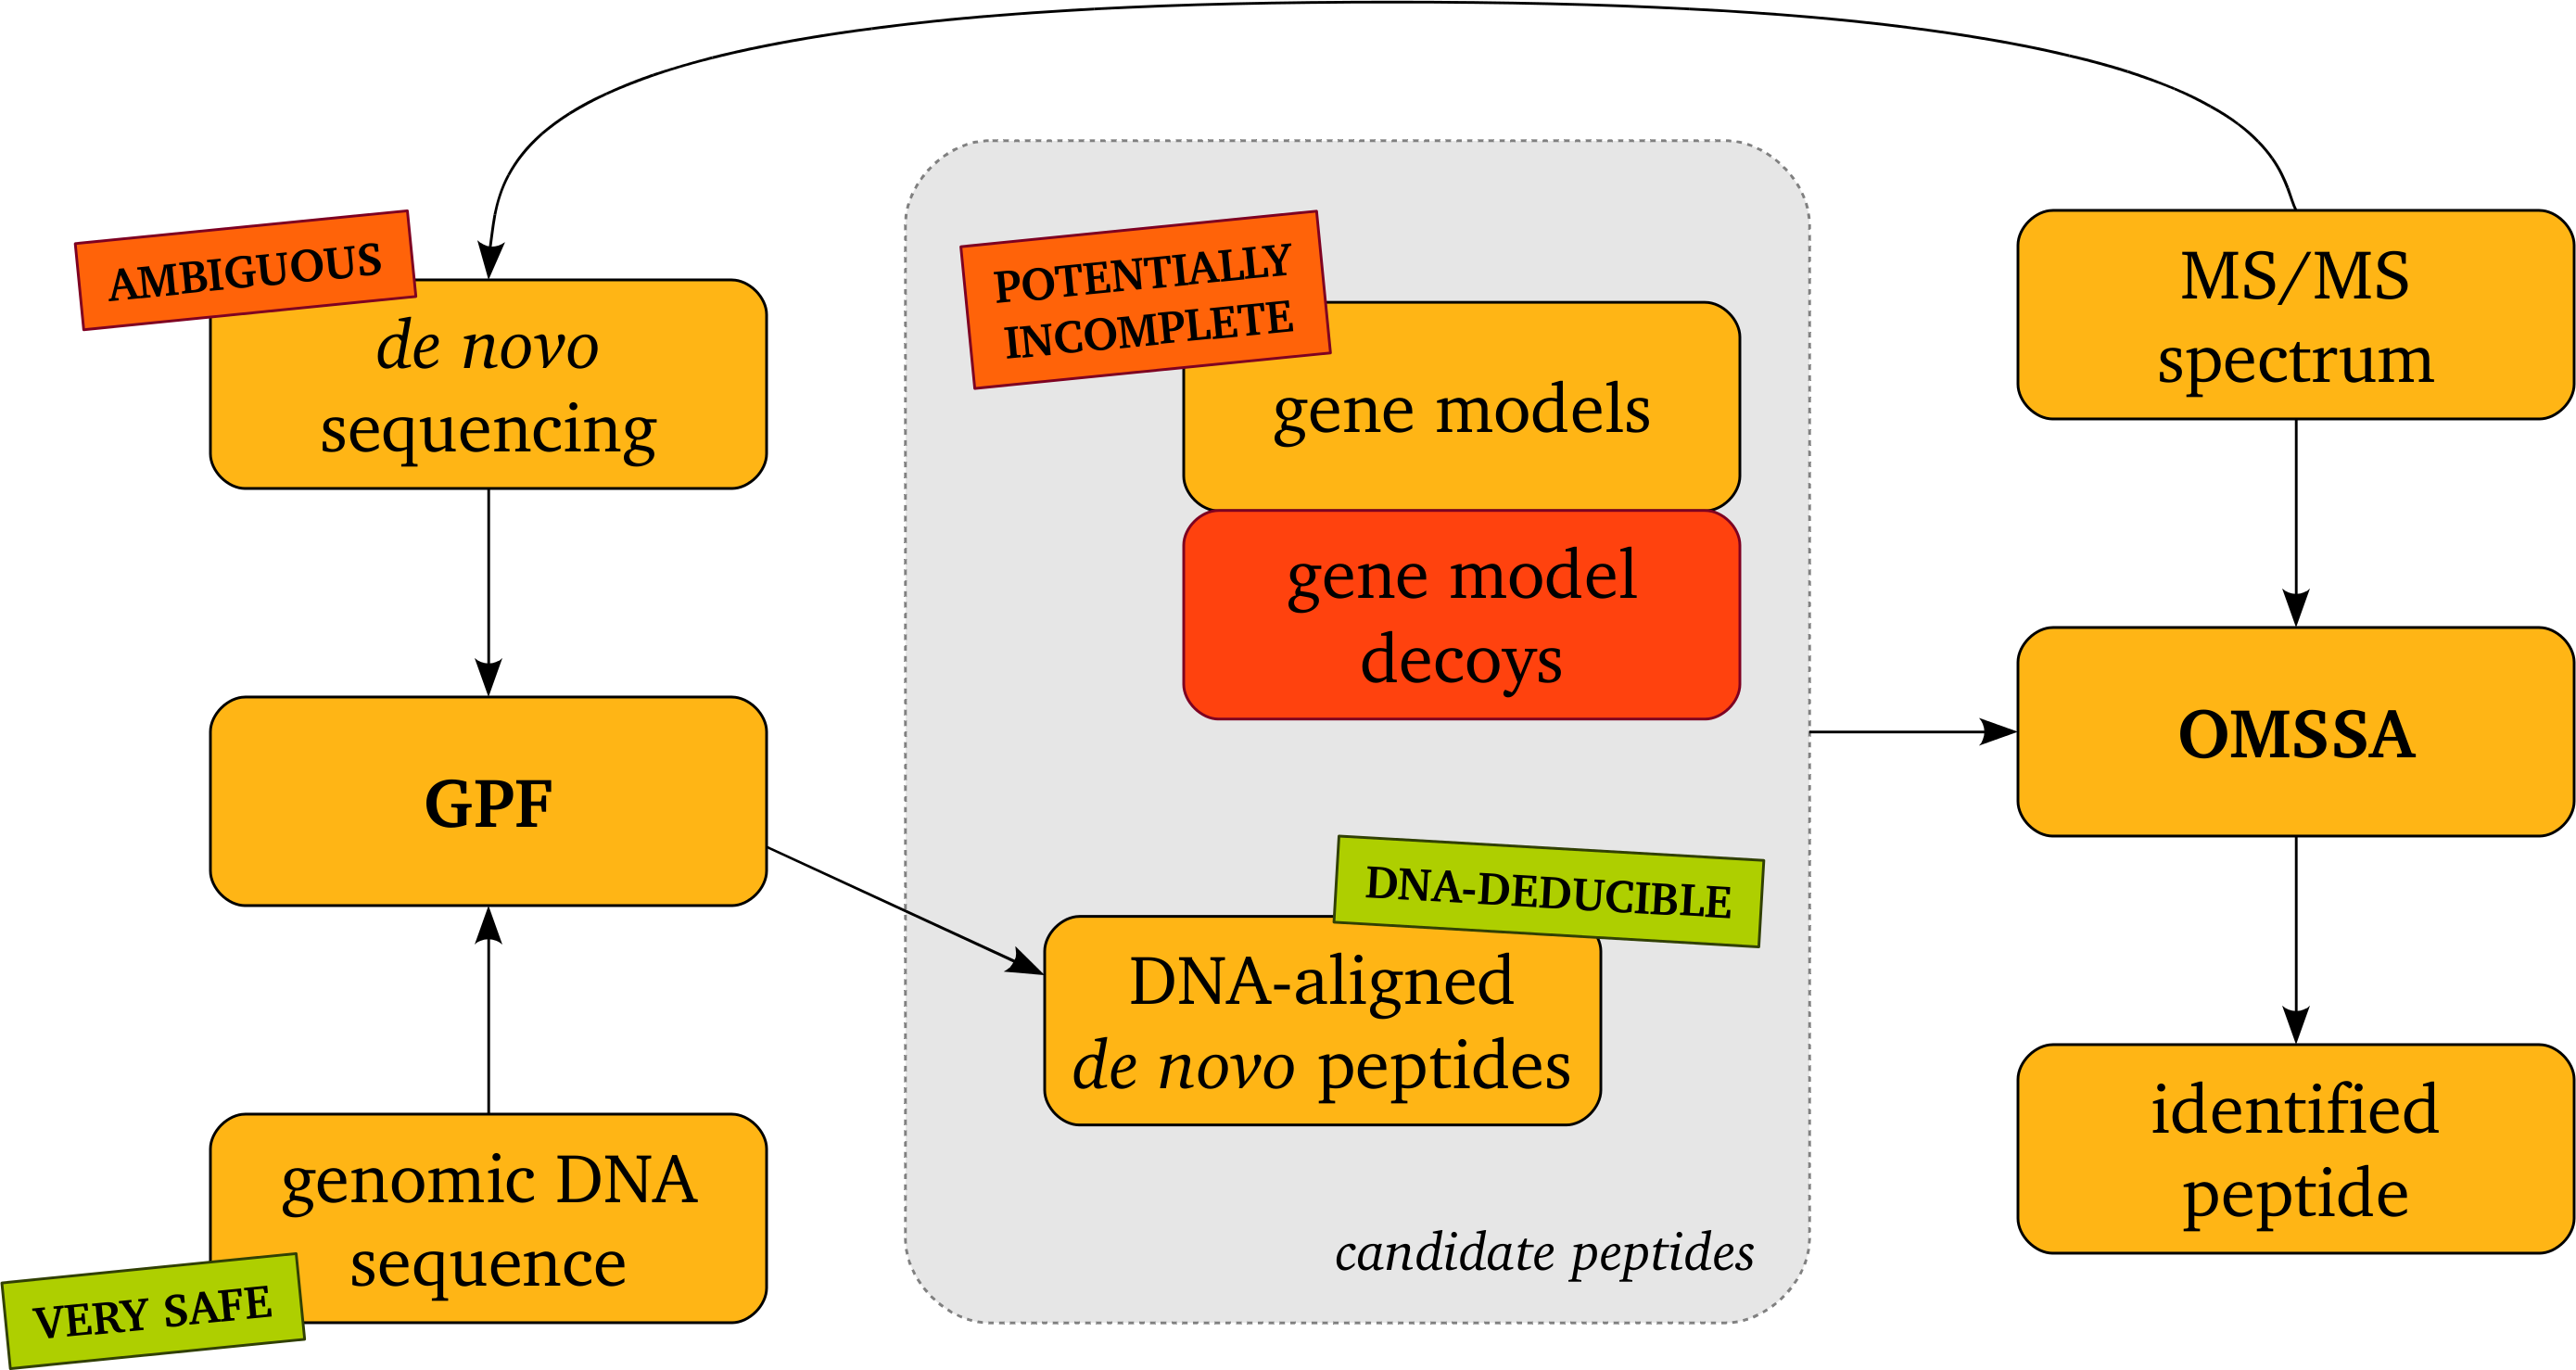
\includegraphics[width=0.7\textwidth]{figures/gpf-omssa.jpg}
\caption{
{\bf Validation of GPF candidate peptides via a target/decoy approach
    using previously established gene models.} 
    Statistical significance of identified GPF candidate peptides is 
    assessed using existing gene models which may be incomplete but
    can be expected to contain a high amount of correct sequences.
}
\label{fig:gpf-omssa}
\end{SCtopfig}

The GPF annotation pipeline presented in this thesis follows a similar strategy
(\cite{Specht2011_GPF}, see p.~\pageref{section:gpf} and \pageref{paper:gpf}).
However, the GPF approach is less biased in comparison to the exon splice graph
approach because it does not require exon/intron prediction as a first step.
GPF candidate peptides are solely generated from MS/MS {\em de novo} sequencing
and subsequent mapping of the resulting peptides to the genome, using 
a user-defined maximum intron length and a set of possible splice donor/acceptor 
site consensus sequences.
This means that intron prediction is carried out on a per-peptide basis, and
all peptides are treated independently.
The actual validation of extrinsic hints and splice site detection is
carried out by AUGUSTUS in the final annotation step.
Moreover, the approach is highly flexible because no specialized database
search program is required because candidate peptides are inferred by GPF
and then passed down the evaluation pipeline alongside a protein database
(see Fig.~\ref{fig:gpf-omssa}).
Although the protein database is used to estimate the FDR of peptide 
identifications, the final GPF-deduced peptides which are exported as
peptide hints do not originate from this database, although in the case
of \cre, a big portion of these protein database peptides could be 
independently confirmed via GPF \citep{Specht2011_GPF}.


\subsection{Proteogenomic genome annotation}

\subsection{Identification of novel targets for reverse-genetics approaches}


% \cleardoublepage
\cleardoublepage
% ==============================================================
\chapter{Summary}
% ==============================================================

A novel platform for the evaluation of mass spectrometric data has been
established and was subsequently employed for the evaluation of measurements
performed to characterize the chloroplast proteome of \cre~and elucidate
its anaerobic response.
Proteomatic provides user-friendly access to mass spectrometric data 
evaluation programs and allows for the construction of complex workflows.

In order to facilitate the large-scale characterization of the \cre~chloroplast
proteome, qTrace has been designed and implemented to automate the peptide and 
protein quantitation process in full scans.
qTrace supports a variety of metabolic labeling strategies and has 
confirmed the anaerobic induction of proteins previously shown to be induced on
the transcript level.
Furthermore, several proteins of unknown function have been found induced
under anaerobic conditions which represent interesting targets for further 
research.

{\em De novo}-based peptide sequencing is a powerful approach for the annotation
of MS/MS spectra, complementing gene model-supported database search algorithms.
The inherent ambiguity of {\em de novo} sequenced peptides is greatly diminished
by the Genomic Peptide Finder which matches the potentially erroneous
peptide sequences to the genomic DNA sequence of an organism, thereby discarding
spurious peptides and correcting erroneous {\em de novo} sequences.
A new version of the Genomic Peptide Finder, improved in terms of sensitivity, 
specificity, and search speed has been presented in this thesis.

Furhermore, a method for the automated statistical validation of GPF peptides
has been developed and has led to the possibility of using GPF peptides as
an extrinsic hint source for the {\em ab initio} gene prediction program 
AUGUSTUS in a high-throughput proteogenomic genome annotation pipeline.

All software developed in the scope of this thesis is publicly available
at \href{http://github.com/specht}{http://github.com/specht}.


% \cleardoublepage
% ==============================================================
\chapter*{Appendix A: qTrace -- Rapid quantitation of metabolically labeled sister peptides}
\markboth{Appendix A: qTrace -- Rapid quantitation of metabolically labeled sister peptides}{Appendix A: qTrace -- Rapid quantitation of metabolically labeled sister peptides}
\addcontentsline{toc}{chapter}{Appendix A: qTrace -- Rapid quantitation of metabolically labeled sister peptides}
% ==============================================================

In addition to identification, peptide and protein quantitation via mass 
spectrometry has become an important aspect of mass spectrometric analysis 
\citep{Kline2010, Schulze2010}. 
Various programs for peptide and protein quantitation in metabolically labeled 
samples have been published \citep{Han2001, Li2003, Saito2007, Park2008, 
Cox2008, Mortensen2010}, with different platform support and label handling 
capabilities. 
However, none of these tool provides operating-system independent support
for various metabolic labeling strategies.
To overcome this, qTrace, a novel quantitation software has been 
created in the scope of this thesis.
Like OMSSA, qTrace can be 
used within Proteomatic.
qTrace searches for the isotope envelopes of previously identified sister 
peptides in MS1 full scans and allows for various labeling strategies, 
including stable isotopic labeling by amino acids in cell culture (SILAC) 
and \textsuperscript{15}N labeling.

\section*{Quantitation workflow}

qTrace uses a list of peptides which have been previously identified via MS/MS
(`target peptides') and performs peptide quantitation based on the corresponding 
precursor ions in full scans.
Users may choose from a list of predefined labels or manually specify a 
labeling strategy using a syntax which accurately describes the label applied 
to the sample.
Labels can be defined by specifying certain isotopes such as `15N' or `13C'.
Combinations of multiple isotopes are possible. 
Isotopes may be followed by a labeling efficiency: `15N (0.994)'
indicates that 99.4\% of all nitrogen atoms in the labeled sample are 
\textsuperscript{15}N isotopes, and the remaining 0.06\% are 
\textsuperscript{14}N isotopes. 
Isotopes, or combinations thereof, may be prefixed with an 
amino acid scope that constrains isotopes to certain amino acids: 
`R 13C' indicates \textsuperscript{13}C atoms in all arginine residues (like for 
isotopes, multiple amino acids may be specified). 
To accommodate for the effect that labeled arginine residues may lead 
to labeled proline residues due to their shared amino acid biosynthesis pathways, 
variable labels may be defined by suffixing an amino acid with the star 
symbol: `RP* 13C' indicates heavy carbon atoms in all arginine residues 
and also variably in all proline residues, leading to $n$ additional labeled 
isotope envelopes, where $n$ is the number of proline residues in the target peptide.
Finally, an amino acid scope may be negated by using the caret symbol: 
`$\caret$R 15N' indicates \textsuperscript{15}N isotopes in all residues 
except arginine.

\section*{Abundance estimation}

qTrace offers two modes of abundance estimation: (a) a {\em fixed peak count} 
mode and (b) an {\em isotope envelope fitting} mode. 

In the {\em fixed peak count} mode, a fixed number of required isotope peaks $n$,
including the monoisotopic peak, is defined by the user.
qTrace calculates the {\em m/z} values of the respective isotope peaks 
\mbox{$A+0$} to $A+(n-1)$ for every unlabeled and labeled target peptide within 
a user-definable charge state range and stores these target peaks as 
`required present'. 
In addition, the $A-1$ peak of the light sister peptide is stored as 
`required absent', because its presence for one peptide would imply 
that its alleged $A+0$ peak might in fact be the $A+i$ peak of 
another peptide. 
The calculated {\em m/z} values are then matched to the observed {\em m/z} 
values within a user-defined precursor mass tolerance.
Whenever all presence and absence requirements are met for a certain unlabeled 
or labeled peptide, its abundance is estimated by summing the peak heights of 
all peaks stored as `required present'. 

Using the {\em isotope envelope fitting} mode, peak intensities are calculated in 
addition to the {\em m/z} values by predicting the shape of the 
isotope envelope from the elemental composition of every target peptide. 
Instead of defining a fixed number of isotope peaks per precursor ion, `required
present' peaks are defined using a relative intensity threshold in respect to the
highest peak of the predicted isotope envelope.
This leads to a variable `required isotope peak' count per peptide, depending on 
its elemental composition.
Typically, a relative intensity threshold of 50\% is used to define `required 
present' peaks. 

\begin{figure}
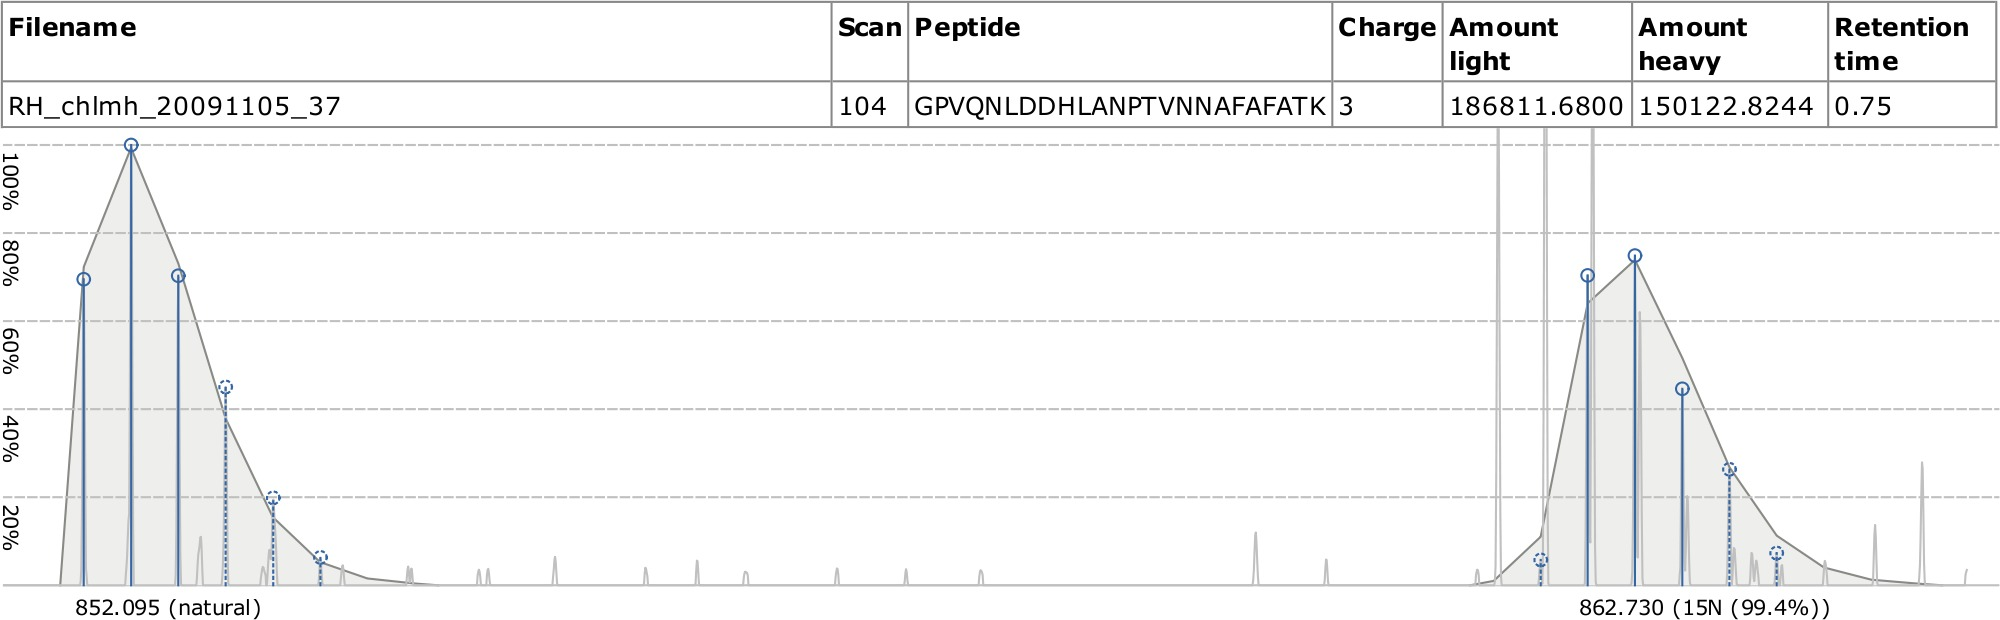
\includegraphics[width=\textwidth]{figures/qtrace-figure.jpg}
\caption{
    {\bf An example sister peptide pair from a 
    \textsuperscript{14}N/\textsuperscript{15}N labeled 
    {\em C. reinhardtii} sample as observed in a MS1 full scan. }
    {\em Required} peaks with a relative peak intensity of at least 50\% are 
    denoted by solid circled lines, {\em considered} peaks with a relative peak 
    intensity of at least 1\% are denoted by dashed circled lines. 
    The areas shaded in gray depict the theoretical isotope envelopes fitted to
    the observed {\em required} and {\em considerded} peaks and yield a light/heavy
    ratio of 1.24 for this scan.}
\label{fig:qtrace}
\end{figure}

All `required present' peaks have to be present in the spectrum for the peptide 
to be identified.
In addition, a variable number of `considered if present' peaks may be defined
via a second threshold (typically 1\%). 
All `required present' and `considered if present' {\em m/z} values are matched 
to the observed {\em m/z} values.
If all required peaks are present in the scan, the union of all `required' and
`considered' peaks is fitted to the theoretical isotope envelope, taking peak
heights into account.
A fitting error is determined and used to discard false matches.
Because the shape of the theoretical isotope envelope is taken into account, 
it is not necessary to check for the absence of the unlabeled $A-1$ peak.
The area under the fitted isotope envelope is then used as an estimate for
peptide abundance (see Fig.~\ref{fig:qtrace}).

\section*{Result compilation}

For demonstration purposes, the following experimental context is assumed:
\textsuperscript{14}N/\textsuperscript{15}N differentially labeled proteins from 
the unicellular green alga {\em Chlamydomonas reinhardtii} were mixed at equal 
protein concentration and fractionated by SDS-PAGE. After separation, protein 
bands were excised, digested with trypsin and analyzed by liquid chromatography 
coupled mass spectrometry.
Data evaluation of the resulting full and fragmentation scans was conducted via 
Proteomatic using OMSSA for identification and qTrace for quantitation. 

The output of qTrace is a list of peptide quantitation events in full scans.
Every quantitation event denotes unlabeled and labeled abundances of a peptide 
in a defined context (e.g. certain SDS-PAGE band and/or retention time),
at a certain charge state.
In the context of qTrace, the combination of peptide, band, and charge is called 
the {\em PBC combination} of a certain quantitation event.
Ratios are determined by dividing the sums of all unlabeled and labeled peptide
abundances within a PBC combination to accomodate for small retention time
shifts of sister peptides.
In addition, different PBC combinations can be regarded as independent observations 
of the peptide over retention time and a minimal PBC combination count can therefore 
be used as a filter criterion in a subsequent processing step.

The following filtering steps are provided by Proteomatic (see Fig.~\ref{fig:exp-setup}):

{\bf Add protein information.}
For every peptide quantitation event, the corresponding protein (or
protein group) is determined, and all quantitation events of peptides 
appearing in multiple proteins (or protein groups) are discarded.

\begin{figure*}
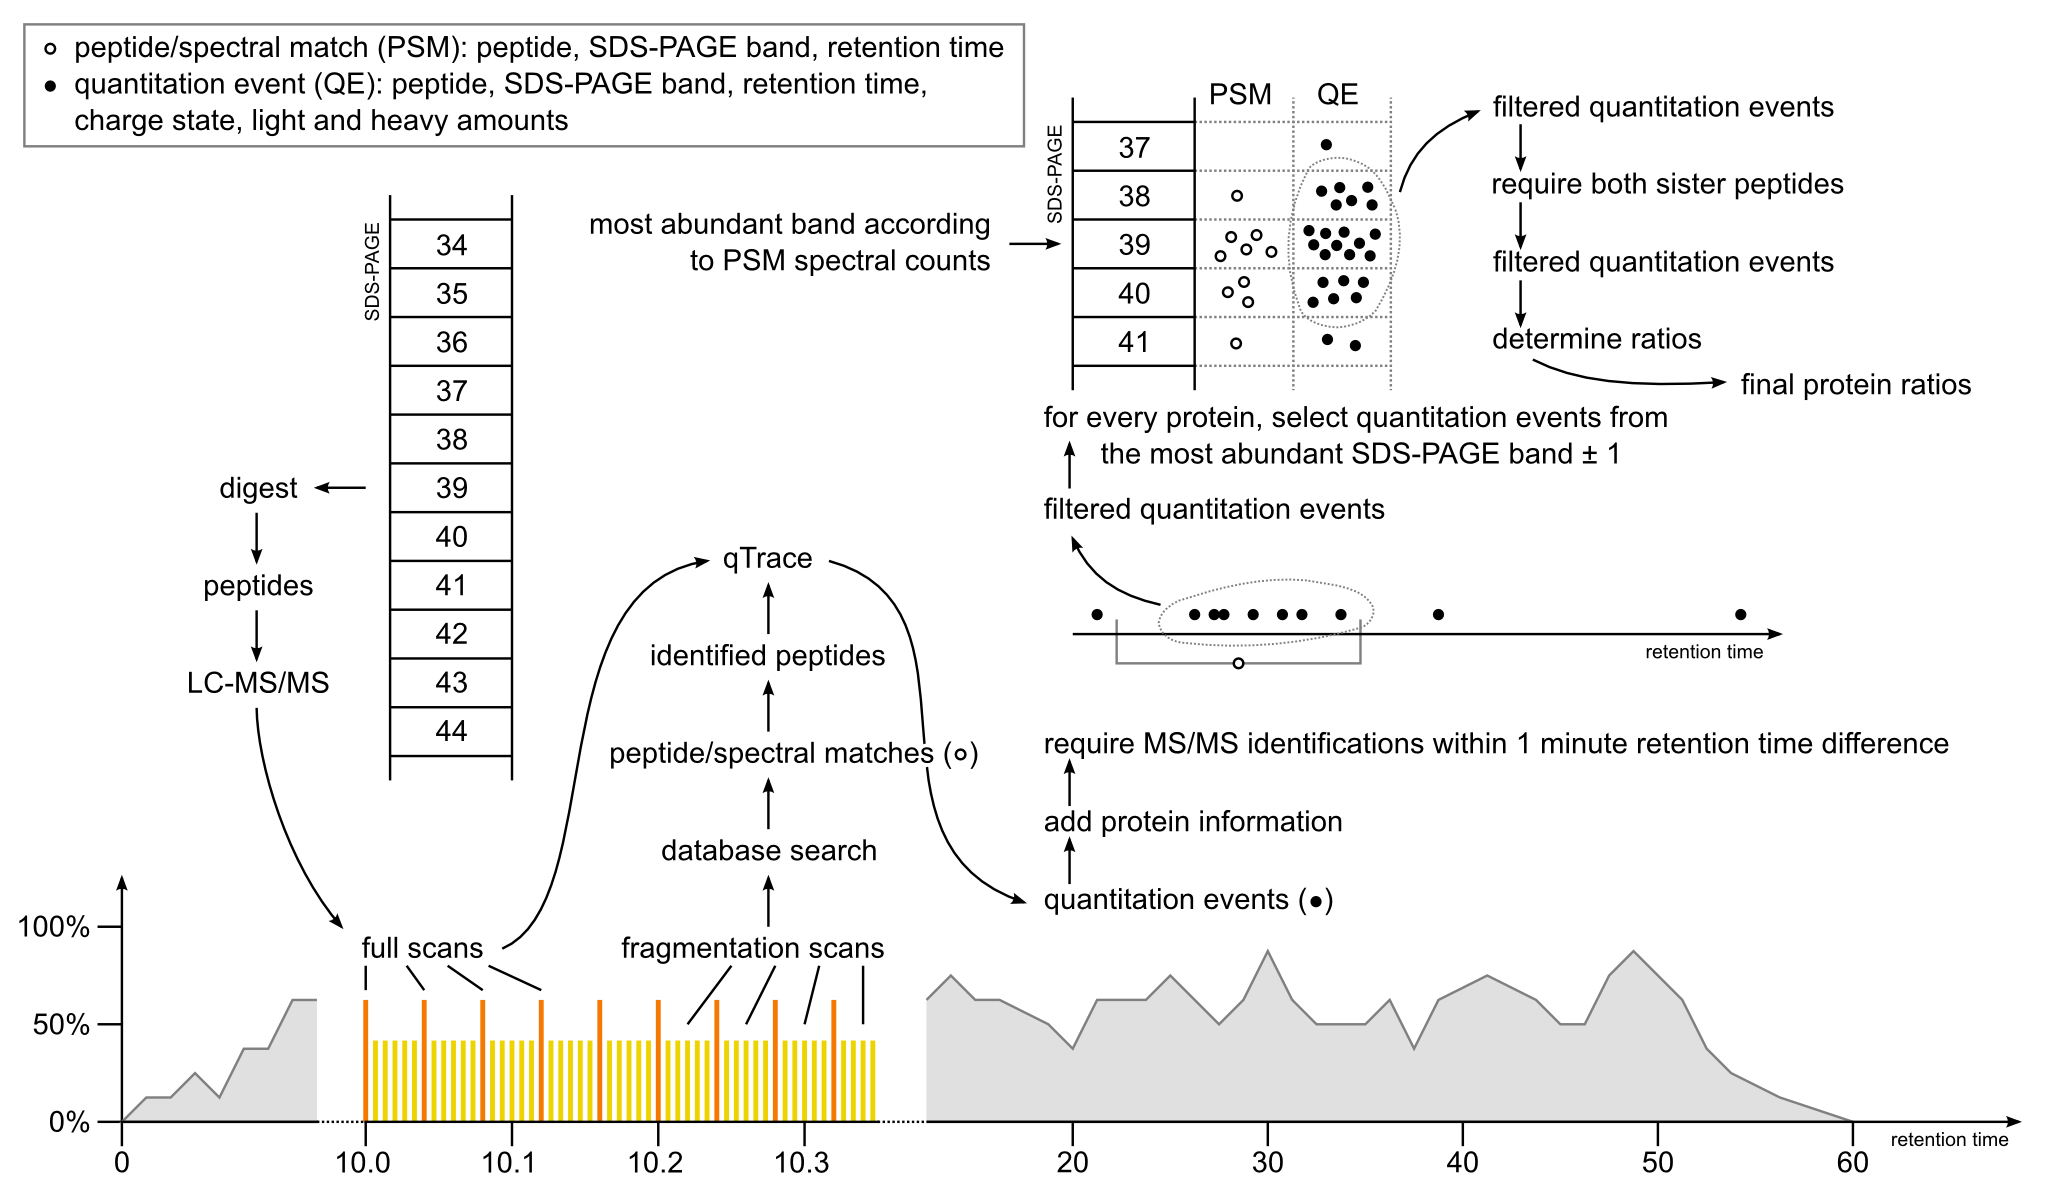
\includegraphics[width=\textwidth]{figures/exp-setup.jpg}
\caption{
    {\bf Depiction of the experimental workflow for protein identification and 
    quantitation. }
    Protein samples are subjected to two steps of separation: (a) SDS-PAGE, in 
    which each sample is fractionated into distinct bands, and (b) HPLC, which 
    separates the digested peptides from each SDS-PAGE band according to their 
    hydrophobicity. 
    The peptides eluting from the HPLC are measured using the {\em Big 5} 
    method which produces full scans and fragmentation scans in an interleaved 
    pattern. 
    While the fragmentation scans are used to identify peptides via a database 
    search (e. g. using OMSSA), the full scans are used by qTrace to quantify 
    the previously identified peptides using their light and heavy precursor 
    masses.
    The resulting quantitation events (QE) are then filtered in such a way
    that MS/MS identifications are required within a short retention time 
    difference. 
    The peptide quantitation events are compiled to protein quantitation events
    by determining which protein a peptide belongs to and discarding all events
    from ambiguous peptides.
    In addition, the spectral counts derived from the MS/MS identifications are 
    used to determine the SDS-PAGE band in which a protein has been must 
    abundantly identified in, and only quantitation events from this band 
    ($\pm$1) are accepted.
    Finally, the protein ratios are determined.
}
\label{fig:exp-setup}
\end{figure*}

{\bf Require MS/MS identifications.}
All quantitation events for which no MS/MS identification exists in the same 
SDS-PAGE band within a user-defined retention time difference (1 minute by 
default) are discarded. This filter corresponds to the separation of the 
tryptic peptides via liquid chromatography.

{\bf Pick most abundant SDS-PAGE band.}
For every protein, the SDS-PAGE band in which the protein has been identified 
in most abundantly is determined, and only quantitation events stemming from 
this band ($\pm$ a user-defined tolerance, typically 1) are discarded. This 
filter corresponds to the fractionation step via SDS-PAGE.

{\bf Require both sister peptides.}
Quantitation events in which only one of the sister peptides (labeled or 
unlabeled) could be quantified can be considered less reliable than quantitation 
events in which both sister peptides could be quantified.
This is because the missing peptide might have escaped detection due to a 
post-translation modification resulting in a different precursor mass. 
This filter rejects all quantitation events in which one sister peptide has 
been quantified with an abundance of zero.

{\bf Determine ratios.}
In all previous processing steps, only abundances have been determined and 
filtered. 
This step determines actual ratios by dividing the sums of unlabeled and 
labeled abundances within every PBC combination and then determining the final 
protein ratio as the mean (and standard deviation) of the individual PBC 
combination ratios.
A high number of PBC combination ratios is favorable because every PBC 
combination may be regarded as an independent observation of a sister peptide 
pair.


% \cleardoublepage
% ==============================================================
\chapter*{Appendix B: Proteomatic workflow for proteogenomic genome annotation}
\markboth{Appendix B: Proteomatic workflow for proteogenomic genome annotation}{Appendix B: Proteomatic workflow for proteogenomic genome annotation}
\addcontentsline{toc}{chapter}{Appendix B: Proteomatic workflow for proteogenomic genome annotation}
% ==============================================================

% ==============================================================
\renewcommand{\baselinestretch}{1.0} 
\renewcommand{\arraystretch}{1.0} 
% ==============================================================

\begin{figure}
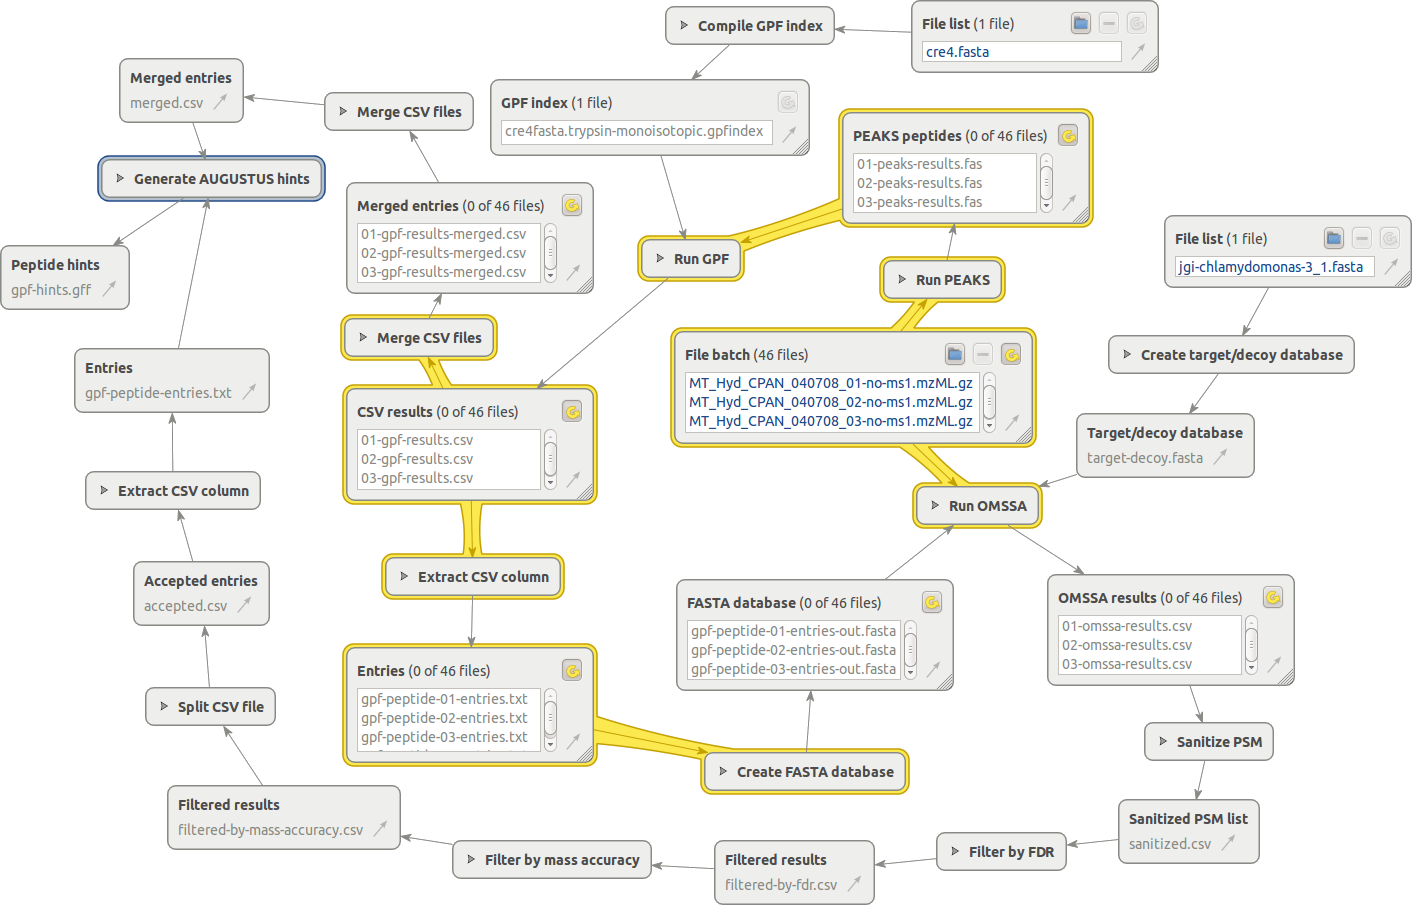
\includegraphics[width=\textwidth]{figures/gpf-annotation.jpg}
\label{fig:gpf-annotation}
\end{figure}


\newpage
\bibliography{library}
\addcontentsline{toc}{chapter}{References}
\markboth{References}{References}
% \bibliographystyle{abbrvnat-no-url}
\bibliographystyle{bst}
    
\cleardoublepage
% ==============================================================
\chapter*{Acknowledgements}
\markboth{Acknowledgements}{Acknowledgements}
\addcontentsline{toc}{chapter}{Acknowledgements}
% ==============================================================

First of all, I would like to thank
Michael Hippler for giving me the opportunity to explore the field of
mass spectrometry-based proteomics which presented me with a multitude
of opportunities to solve problems and develop computational strategies.
It has been an incredibly good experience and I have learned a lot.

I would furthermore like to thank:

\begin{itemize}
\item
Sebastian Kuhlgert who explained biochemistry and photosynthesis to me in a 
way that acknowledged my previous experience in the field which was close to 
nil, and impressed me with his smooth working style at the lab bench
whenever I had the chance to watch,

\item
Mia Terashima who I shared a lot of headaches with during many iterations of 
writing and revising manuscripts which turned out to be much easier to cope
with using leetspeak,

\item
Kerstin Trompelt, Ingrid Janßen and Andreas Busch who took me into the lab for
two weeks and made me carry out what felt like hundreds of tasks on \cre~samples 
before the spectral files were finally written to disk which was were I started
to feel more comfortable again,

\item
Jule Wolf who asked lots of questions and wanted to understand protein groups so 
badly that she plastered an entire wall with {\em post-it note} peptides and then
arranged them into proteins and protein groups, which helped,

\item
Jens Allmer who had the original vision of an easy-to-use proteomics data evaluation 
platform,

\item Christian Fufezan who introduced me to Python and showed me that it is possible 
after all to have the cake and eat it, too,

\item
the people who have spent time on improving and extending Proteomatic:
Sebastian Kuhlgert, Christian Fufezan, Till Bald, Phillip Ihmor and Johannes Barth,

\item
Andreas Schaaf who showed me around a lot during my first months and made me 
capable of telling a washing basin from a fermenter,

\item
Martin Scholz who shares a curious affection for trivia from the last decades of 
the twentieth century with me,

\item
all the incredibly patient people who explained the molecular biology 101 to me 
again and again -- and then again:
Frank Bernard,
Susan Hawat,
Marita Hermann,
Ricarda Höhner,
Bernadeta Kukuczka,
Bianca Naumann, 
Elisabeth Ostendorf,
Dimitris Petroutsos and Irina Tolstygina.

\end{itemize}

Finally, I would like to thank my wife, Jule, who is always full of splendid ideas
and plans that tend to work out.
Last but not least I would like to say thanks to my children, Charlotte and Leo, 
who force me to take a step back from work on a regular basis and acknowledge that 
what's important to somebody is highly subjective.


\cleardoublepage
% ==============================================================
\chapter*{Curriculum vitae}
\markboth{Curriculum vitae}{Curriculum vitae}
\addcontentsline{toc}{chapter}{Curriculum vitae}
% ==============================================================

% Michael Specht \\
% Toppheideweg 34 \\
% 48161 Münster
% 
% Phone: +49 251 4808158 \\
% E-mail: \href{mailto:michael.specht@uni-muenster.de}{michael.specht@uni-muenster.de}
% 

\begin{longtable}{@{}lp{12.5cm}}

\cvsubheader{Personal details}

Date of birth: & December 23, 1981 \\
Place of birth: & Magdeburg, Germany \\
Marital status: & married, two children\\
\\

\cvsubheader{Publications}

04/2011 & Terashima M., {\bf Specht M.}, Hippler M. (2011). The chloroplast proteome: A survey from the {\em Chlamydomonas reinhardtii} perspective with a focus on distinctive features. Current Genetics 2011 (in press). \\%; DOI: \href{http://dx.doi.org/}{} (in press). \\

03/2011 & {\bf Specht M.}, Stanke M., Terashima M., Naumann-Busch B., Janßen I., Höhner R., Hom E. F. Y., Liang C., Hippler M. (2011). Concerted action of the new Genomic Peptide Finder and AUGUSTUS allows for automated proteogenomic annotation of the Chlamydomonas reinhardtii genome. Proteomics 2011; doi: \href{http://dx.doi.org/10.1002/pmic.201000621}{10.1002/pmic.201000621} (in press). \\

02/2011 & {\bf Specht M.}, Kuhlgert S., Fufezan C., Hippler M. (2011). Proteomics to go: Proteomatic enables the user-friendly creation of versatile MS/MS data evaluation workflows. Bioinformatics (2011) 27 (8): 1183-1184; doi: \href{http://dx.doi.org/10.1093/bioinformatics/btr081}{10.1093/bioinformatics/btr081}. \\

07/2010 & Terashima M., {\bf Specht M.}, Naumann B., Hippler M. (2010). Characterizing the anaerobic response of Chlamydomonas reinhardtii by quantitative proteomics. Mol Cell Proteomics, 9(7), 2010: 1514-32; doi: \href{http://dx.doi.org/10.1074/mcp.M900421-MCP200}{10.1074/mcp.M900421-MCP200}. \\

08/2009 & Fufezan C., {\bf Specht M.} (2009). p3d – Python module for structural bioinformatics. BMC Bioinformatics (2009) 10:258; doi: \href{http://dx.doi.org/10.1186/1471-2105-10-258}{10.1186/1471-2105-10-258}. \\

11/2007 & Ropinski T., {\bf Specht M.}, Meyer-Spradow J., Hinrichs K., Preim B. (2007). Surface Glyphs for Visualizing Multimodal Volume Data. Vision, Modelling and Visualization (VMV) (3-13), Saarbrücken, 2007. \\

\newpage 

\cvsubheader{Talks}

\cvtitle{03/2011}{DGMS 2011, Dortmund}
& Proteomics to go: Proteomatic enables the user-friendly creation of versatile MS/MS data evaluation workflows. \\
\tabspace\\


\cvsubheader{Professional experience}

\cvtitle{since 04/2007}{Institute of Plant Biology and Biotechnology\newline Westfälische Wilhelms-Universität Münster}
& Doctoral student in the lab of Prof. Dr. Michael Hippler \newline
% \vspace{6pt}
\vspace{-9pt}
\begin{compactitem}
\item Proteomatic: design and implementation of a user-friendly, decentralized MS/MS data 
evaluation platform \vspace{4pt}\newline
Link: \href{http://www.proteomatic.org}{http://www.proteomatic.org}
% \vspace{-12pt}
% \begin{compactitem}
\item Genomic Peptide Finder: Software for the alignment of MS/MS {\em de novo}
predicted amino acid sequences to the genomic DNA sequence of an organism.
Resulting peptides may be used for evidence-based proteogenomic genome annotation. \vspace{4pt}\newline
Link: \href{http://github.com/specht/gpf}{http://github.com/specht/gpf}.
\item qTrace: Software for the high-throughput quantitation of metabolically
labeled samples (e.g. $^{\textrm{13}}$C Arg SILAC or $^{\textrm{15}}$N) in survey scans.\vspace{4pt}\newline
Link: \href{http://github.com/specht/qtrace}{http://github.com/specht/qtrace}
% \end{compactitem}
\item establishment of free MS/MS data evaluation software in the lab, resulting 
in increased throughput, lower costs and proliferation of MS/MS data 
evaluation-related expertise
\end{compactitem}
% \vspace{-6pt}
\tabspace\\

\cvtitle{10/2006 -- 03/2007}{PROVISIO Software GmbH Münster}
& Software developer -- Realtime Rendering Group \newline
\vspace{-9pt}
\begin{compactitem}
\item design and implementation of a fast JPEG decoder
\item implementation of various user interface widgets for Pictomio
(photo viewer software)
\end{compactitem}
\vspace{-6pt}
\tabspace\\

\cvtitle{07/2005 -- 02/2006}{1komma6 Multimediale Dienstleistungen GmbH Münster}
& Internship -- Web development, focus on accessibility \newline
\tabspace\\

\newpage

\cvsubheader{Education}
\cvtitle{03/2006 -- 11/2006}{Diploma thesis}
& \emph{Glyph-enhanced Volume Visualization}. \newline
Development of a visualization method for the interactive, simultaneous display 
of multiple, related medical data sets (CT and PET).\tabspace\\
% % \input{../../common-en/chromacoding}
% % \input{../../common-en/studienarbeit}
% 

\cvtitle{10/2001 -- 11/2006}{Study of Computational Visualistics}
& Study of Computational Visualistics (computer science with a focus on computer 
graphics) at the Otto-von-Guericke-Universität Magdeburg.\tabspace\\

\cvtitle{09/2000 -- 07/2001}{Alternative civilian service}
& Civilian service at the retirement home "`Luisenhaus"', Potsdam. \tabspace\\

\cvtitle{09/1992 -- 05/2000}{Secondary school}
& Werner-von-Siemens-Gymnasium, Magdeburg. \tabspace\\

% 
% \newpage
% 
\cvsubheader{Further education}
% 
\cvtitle{10/2010}{Advanced Scientific Programming in Python}
& Participated in an autumn school, held in Trento, Italy,
organized by G-Node, the center for Mind/Brian Sciences, and Fondazione Bruno Kessler.\tabspace\\

\newpage

% \cvsubheader{Miscellaneous projects}
% % 
% % % \input{../../common-en/nprflow}
% % % \input{../../common-en/hamster}
% % % \input{../../common-en/tutorium}
% % % \input{../../common-en/vib}
% 
% \cvtitle{02/2003}{Student anti war group}
% & Foundation of the student anti war group at the University of Magdeburg,
% shortly before the beginning of the Iraq war in March 2003.
% Planning and organization of discussion rounds and movie nights. \tabspace\\
% 
% \cvtitle{11/2002 -- 11/2003}{Short film "`pixelle ma belle \#01"'}
% & \begin{compactitem}
% \vspace{-9pt} 
% \item design and implementation of a distributed video rendering software
% \item development of an alternative, low-cost blue screen method
% \end{compactitem}
% \vspace{6pt} 
% Link: \href{http://www.pixellemabelle.de}{www.pixellemabelle.de}
% \tabspace\\
% 
% % % \input{../../common-en/fx}
% % % \input{../../common-en/ferienlager}
% % % \input{../../common-en/zeitnahme}
% % 
% \cvsubheader{Skills}
% % 
% 
% foreign languages
% & English (fluent)\newline
% French (basic knowlegde) \tabspace\\
% 
% programming
% & C, C+\kern-0.2em +, Qt, Ruby, Python, PHP, Java, Assembler, XHTML, CSS, Ajax, MySQL\tabspace\\
% 
% software
% & Linux, Windows, Mac OS X \newline
% GIMP, Inkscape, OpenOffice, \LaTeX
% Git, Subversion, CSV\tabspace\\

% 
\end{longtable}
% 



\end{document}
